% System model figure — submission-quality TikZ source.
% Mirrors docs/figures_paper/arch_system_model.png (parameters verified against
% code: N=192 16x12 Walker, lambda_hi=4.0/lo=0.1, ISL B=100-300 Mb/s, F_max=2 GHz,
% E_cap=36 kJ, DoD in [0.1,0.8], DVFS f*=sqrt(Q/3 V_DVFS kappa), H=delta*10^{a(delta-1)}).
% Compiled OK with TeX Live 2023 (pdflatex). Remove the title node when adding a \caption.
%   pdflatex arch_system_model.tex
\documentclass[border=8pt]{standalone}
\usepackage{amsmath}
\usepackage{amssymb}
\usepackage{tikz}
\usetikzlibrary{positioning,arrows.meta,fit,backgrounds,calc,shapes.geometric}

\definecolor{cenv}{HTML}{3F6090}
\definecolor{cact}{HTML}{D62728}
\definecolor{ccri}{HTML}{2CA02C}
\definecolor{cque}{HTML}{7F8C9B}
\definecolor{ctask}{HTML}{B58A00}
\definecolor{csun}{HTML}{E0A800}

\begin{document}
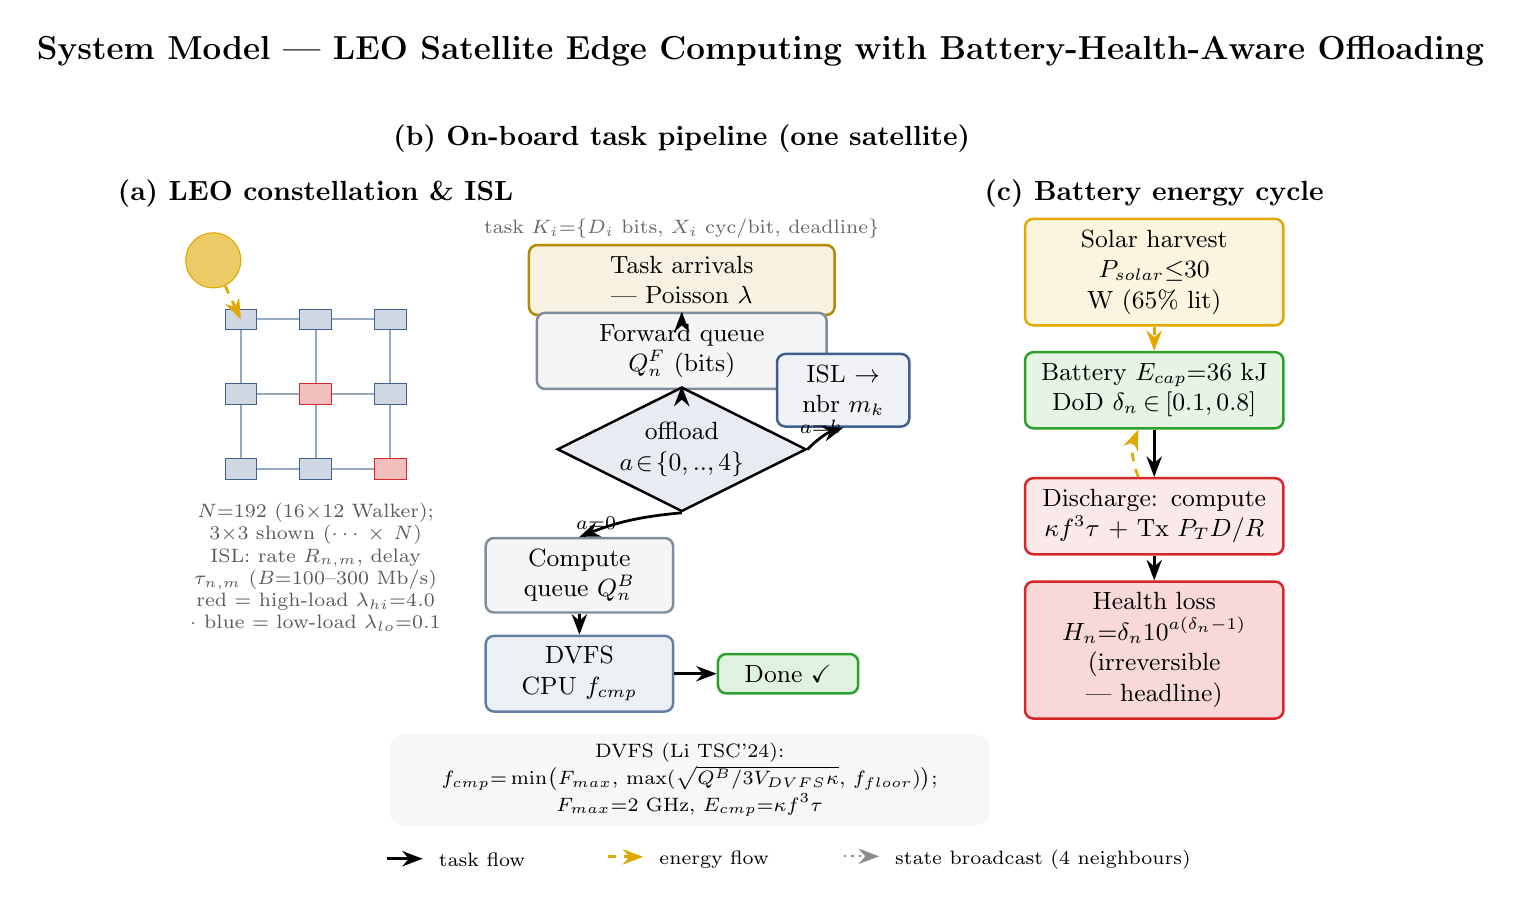
\begin{tikzpicture}[
  font=\small,
  >={Stealth[length=2.6mm]},
  box/.style={rounded corners=3pt, draw, line width=0.9pt, align=center, inner sep=4pt},
  que/.style={box, fill=black!4, draw=cque, text width=3.4cm},
  task/.style={box, fill=ctask!12, draw=ctask, text width=3.6cm},
  cpu/.style={box, fill=cenv!10, draw=cenv!80, text width=2.1cm},
  done/.style={box, fill=ccri!15, draw=ccri, text width=1.5cm},
  bat/.style={box, align=center, text width=3.0cm},
  dec/.style={diamond, aspect=2, draw, line width=0.9pt, fill=cenv!12, align=center, inner sep=1pt},
  sat/.style={rectangle, draw=cenv, fill=cenv!25, minimum width=4mm, minimum height=2.6mm, inner sep=0pt},
  hsat/.style={sat, draw=cact, fill=cact!30},
  taskflow/.style={->, line width=1.0pt},
  eneflow/.style={->, line width=1.0pt, dashed, draw=csun},
  infoflow/.style={->, line width=0.8pt, dotted, draw=black!45},
  note/.style={font=\scriptsize, inner sep=1pt, align=center},
]
\node[font=\large\bfseries] at (6.6,5.3)
  {System Model — LEO Satellite Edge Computing with Battery-Health-Aware Offloading};

% =================== (a) constellation ===================
\begin{scope}[shift={(0,0)}]
  \foreach \i in {0,1,2} \foreach \j in {0,1,2} { \coordinate (s\i\j) at (0.95*\j, 0.95*\i); }
  \foreach \i in {0,1,2} \foreach \j in {0,1} {
    \pgfmathtruncatemacro{\jj}{\j+1} \draw[cenv!55, line width=0.7pt] (s\i\j)--(s\i\jj);}
  \foreach \i in {0,1} \foreach \j in {0,1,2} {
    \pgfmathtruncatemacro{\ii}{\i+1} \draw[cenv!55, line width=0.7pt] (s\i\j)--(s\ii\j);}
  \foreach \i in {0,1,2} \foreach \j in {0,1,2} { \node[sat] at (s\i\j) {}; }
  \node[hsat] at (s11) {}; \node[hsat] at (s02) {};
  \node[circle, fill=csun!60, draw=csun, minimum size=7mm] (sun) at (-0.35,2.65) {};
  \draw[eneflow] (sun) -- (s20);
  \node[note, text=black!65, text width=4.4cm] at (0.95,-1.25)
    {$N{=}192$ (16$\times$12 Walker); 3$\times$3 shown ($\cdots\times N$)\\
     ISL: rate $R_{n,m}$, delay $\tau_{n,m}$ ($B{=}$100--300 Mb/s)\\
     red = high-load $\lambda_{hi}{=}4.0$ · blue = low-load $\lambda_{lo}{=}0.1$};
  \node[font=\bfseries] at (0.95,3.5) {(a) LEO constellation \& ISL};
\end{scope}

% =================== (b) on-board pipeline ===================
\begin{scope}[shift={(5.6,0)}]
  \node[font=\bfseries] at (0,4.2) {(b) On-board task pipeline (one satellite)};
  \node[note, text=black!60, text width=5.2cm] at (0,3.05) {task $K_i{=}\{D_i$ bits, $X_i$ cyc/bit, deadline$\}$};
  \node[task] (arr) at (0,2.4) {Task arrivals — Poisson $\lambda$};
  \node[que] (qf) at (0,1.5) {Forward queue $Q^F_n$ (bits)};
  \node[dec] (dec) at (0,0.25) {offload\\ $a\!\in\!\{0,..,4\}$};
  \node[que, text width=2.1cm] (qb) at (-1.3,-1.35) {Compute queue $Q^B_n$};
  \node[cpu] (cpu) at (-1.3,-2.6) {DVFS CPU $f_{cmp}$};
  \node[done] (done) at (1.35,-2.6) {Done \checkmark};
  \node[box, fill=cenv!8, draw=cenv, text width=1.4cm] (isl) at (2.05,1.0) {ISL $\to$ nbr $m_k$};
  \draw[taskflow] (arr)--(qf);
  \draw[taskflow] (qf)--(dec);
  \draw[taskflow] (dec.south) to[bend right=8] node[note,left,pos=0.6]{$a{=}0$} (qb.north);
  \draw[taskflow] (qb)--(cpu);
  \draw[taskflow] (cpu.east)--(done.west);
  \draw[taskflow] (dec.east) to[bend left=14] node[note,above,pos=0.4]{$a{=}k$} (isl.south);
  \node[note, text width=7.4cm, fill=cenv!5, rounded corners, inner sep=3pt] at (0.1,-3.95)
    {DVFS (Li TSC'24): $f_{cmp}{=}\min\!\big(F_{max},\,\max(\sqrt{Q^B/3V_{DVFS}\kappa},\,f_{floor})\big)$;\quad
     $F_{max}{=}2$ GHz, $E_{cmp}{=}\kappa f^3\tau$};
\end{scope}

% =================== (c) battery cycle ===================
\begin{scope}[shift={(11.6,0)}]
  \node[font=\bfseries] at (0,3.5) {(c) Battery energy cycle};
  \node[bat, fill=csun!12, draw=csun] (solar) at (0,2.5) {Solar harvest\\ $P_{solar}{\leq}30$ W (65\% lit)};
  \node[bat, fill=ccri!12, draw=ccri] (batt) at (0,1.0) {Battery $E_{cap}{=}36$ kJ\\ DoD $\delta_n\!\in\![0.1,0.8]$};
  \node[bat, fill=cact!10, draw=cact] (disc) at (0,-0.6) {Discharge: compute $\kappa f^3\tau$ + Tx $P_T D/R$};
  \node[bat, fill=cact!18, draw=cact] (hl) at (0,-2.3) {Health loss $H_n{=}\delta_n 10^{a(\delta_n-1)}$ (irreversible — headline)};
  \draw[eneflow] (solar)--(batt);
  \draw[eneflow] (disc) to[bend left=22] (batt);
  \draw[taskflow] (batt)--(disc);
  \draw[taskflow] (disc)--(hl);
\end{scope}

% =================== legend ===================
\node[note, anchor=west] at (1.8,-4.95) {\tikz\draw[taskflow](0,0)--(0.45,0); ~task flow};
\node[note, anchor=west] at (4.6,-4.95) {\tikz\draw[eneflow](0,0)--(0.45,0); ~energy flow};
\node[note, anchor=west] at (7.6,-4.95) {\tikz\draw[infoflow](0,0)--(0.45,0); ~state broadcast (4 neighbours)};
\end{tikzpicture}
\end{document}
